\section{Proposed Research}
\label{sec:proposed-work}
The goal of the proposed research is to develop fast,
high-order-accurate, parallel numerical algorithms for large-scale
simulations of the collective hydrodynamics of  amphiphilic particles in a viscous solvent.
%
We have demonstrated that 
our potential theory approach can efficiently simulate self-assembly of 
amphiphilic particles into two-dimensional micelles, bilayer membranes, and vesicles \cite{Fu19}.
%
While these results show great potentials in simulating the collective hydrodynamics of amphiphilic particles and
reproducing mechanical properties of their bilayer assembly, 
several outstanding issues need to be addressed for such approach to be efficiently applied to three-dimensional 
collective hydrodynamics of amphiphilic particles.


\subsection{Specific Aim 1: Elastic properties of amphiphile ensembles}
\label{subsec:specific_aim_1}

\begin{figure}
\begin{center}
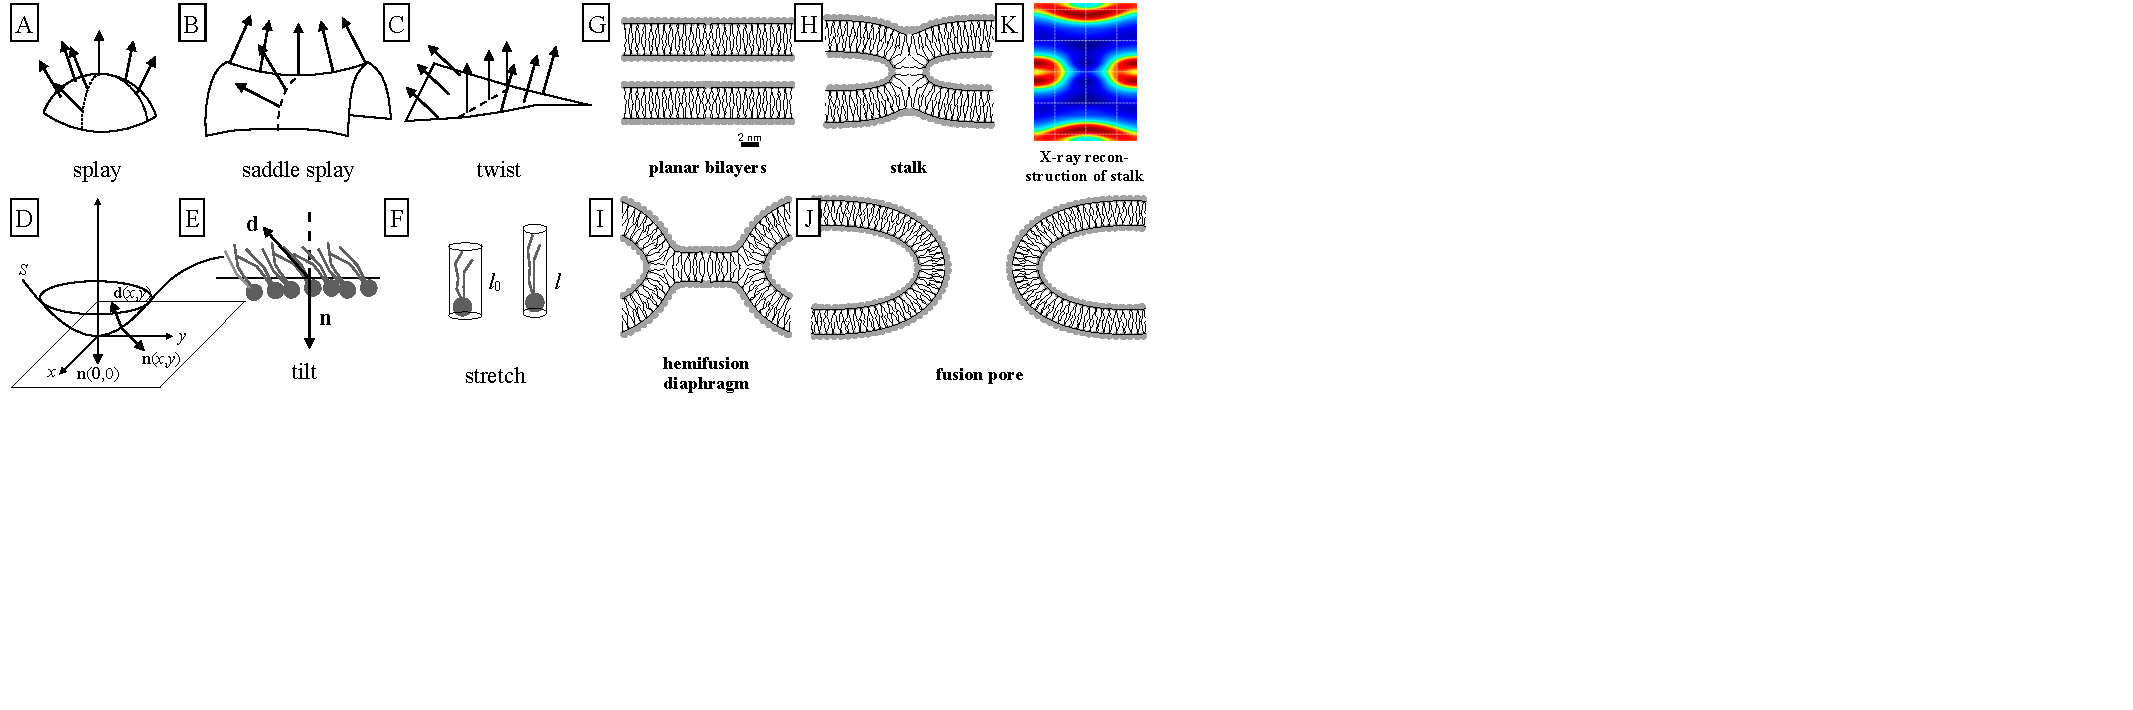
\includegraphics[width=0.9\textwidth]{figures/SA1_fig1.pdf}
\end{center}
\caption{\footnotesize (A--C) The splay ($\Div \mathbf{d}$), 
saddle splay ($\det \mathsf{D}$) and twist ($\Curl \mathbf{d}$) elastic distortions of 
a monolayer. (D) The monolayer neutral surface $\Sigma$,  
director $\mathbf{d}$ and unit normal $\mathbf{n}$ in local coordinates.
(E--F) Lipids are able to tilt from  the surface normal, and stretch.
(H--J) Intermediates of membrane fusion and (K) experimental image of a stalk \cite{Aeffner2012}. }
\label{fig:distortions}
\end{figure}


 We conjecture that 
once assembled, the bilayer shapes possess some or all of the mechanical properties of bilayers from continuum theory. 

The mechanical properties of bilayer are characterized by the Helfrich Hamiltonian;
\begin{equation}
\label{ansatz3}
\begin{aligned}
\int_{\Sigma} 
%&= \tfrac{1}{2}\KB\left[ \left( \tr \mathsf{D} + k_0\right)^2 - k_0^2\right] 
%+ \tfrac{1}{2}\KT (\mathsf{D}_{21} - \mathsf{D}_{12})^2 + \KG  \det \mathsf{D}\\
 \tfrac{1}{2}\KB\left[ \left( \Div \mathbf{d} + k_0\right)^2 - k_0^2\right] 
+ \tfrac{1}{2}\KT (\Curl \mathbf{d})^2 + \KG  \det \mathsf{D} \,dA.
\end{aligned}
\end{equation}
This hamiltonian is the energy functional for one monolayer,
represented by a smooth surface $\Sigma$ and director field $\mathbf{d}$
 \cite{Helfrich73, PhysRevLett.113.248102, Hamm2000}.
The surface $\Sigma$ coincides with the monolayer neutral surface. The 
unit length director $\mathbf{d}$ tracks lipid orientations  
and points from the lipid head toward the lipid tail \cite{doi:10.1021/jp075641w,KLAUDA20083074}.
In a bilayer, the energy is the sum of the two monolayer energies. 
%These monolayers are typically coupled
%by requiring apposing lipid tails to terminate at the same point. 

The form of the elastic energy density \eqref{ansatz3} is the same as
the Oseen-Frank energy density for nematic liquid crystals \cite{ANDRIENKO2018520,Tran7106}.  In fact,  
a lipid monolayer acts as one layer in a smectic  phase \cite{REYESMATEO1995978,Rangamani20140463,PhysRevLett.113.248102}. 
The constants $\KB$, $\KT$  and $\KG$ play the same role as the Frank constants $K_1$, $K_2$ and $K_{24}$
liquid crystal theory. 
The Helfrich hamiltonian derives from the assumption of a quadratic energy density
in the director surface gradient 
$[\mathsf{D}]_{ij} = \frac{\partial \mathbf{d} }{\partial \tau_i} \cdot \tau_j,$ $i,j = 1,2,$ 
where $\tau_1$ and $\tau_2$ are orthogonal tangent vectors. Thus, the 
director gradients in \eqref{ansatz3} couple to surface geometry. 
Symmetries  with respect to mirror reflection and in-plane rotation 
require that the energy come from
\emph{splay} ($\Div \mathbf{d}$), 
\emph{twist} ($\Curl \mathbf{d}$)
or \emph{saddle-splay} ($\det \mathsf{D}$) distortions,
where $\Div$ and $\Curl$ are the surface divergence  and curl  operators, respectively (Figure \ref{fig:distortions}A--C).
The associated elastic coefficients  are the \emph{bending modulus} $\KB$,  \emph{twist modulus} $\KT$ 
and \emph{saddle-splay modulus} $\KG$.

The \emph{spontaneous curvature} $k_0$ depends on lipid composition and determines the preferred lipid splay,
\cite{RoLi15,Kozlov2007}. 
Figure \ref{fig:distortions}A illustrates positive splay. 
The lipid DSPC, for instance, has $k_0 = -0.1$ nm$^{-1}$ 
%as a result of  %having a relatively long acyl chain. 
and these lipids would line the  inner monolayer of a 
spherical liposome, because the addition of a positive splay $\Div \mathbf{d}$  in \eqref{ansatz3}
to the negative spontaneous curvature $k_0$ leads to lower energy \cite{Kamal22245, C3SM51829A, RoLi15,FriedSeguin15}.
The subtraction of $k_0^2$ makes the energy distortion 
free\footnote{The  ``bend'' distortion from nematics  
is not present in monolayers since the directors have no dependence in the normal direction,  \ie the 
Frank ``bend'' constant $K_3$ should not be confused with the \emph{bending modulus} $\KB.$ 
There is also no ``spontaneous twist'' in monolayers due to invariance under mirror reflection.}. 

The Helfrich hamiltonian is widely used to determine energy barriers of fusion between lipid bilayer membranes \cite{ChKo08}. 
%Some of these barrier heights were never before obtained through the use of continuum membrane mechanics.
PI Ryham and collaborators calculated, for the first time in continuum theory, a least energy path for transitions between planar bilayers, a membrane stalk, hemifusion diaphragm and the fusion pore  \cite{RyWaCo13, RyKlYaCo16}. 
%The calculation of hydrophobic 
%fissures in \cite{RyKlYaCo16} motivated the HAP theory. 
These studies 
%analyzed the dependence of energy barriers on
%lipid composition and 
found that each of the transitions required on the order of 30 \kBT\; (Figure \ref{fig:barriers}A),
a result that is in agreement with barrier heights derived by recent molecular dynamics and experimental studies
\cite{FrRoPi17}.  
(Throughout the proposal, \kBT\; = 4.11$\times 10^{-21}$ J.)



\begin{figure}
\begin{center}
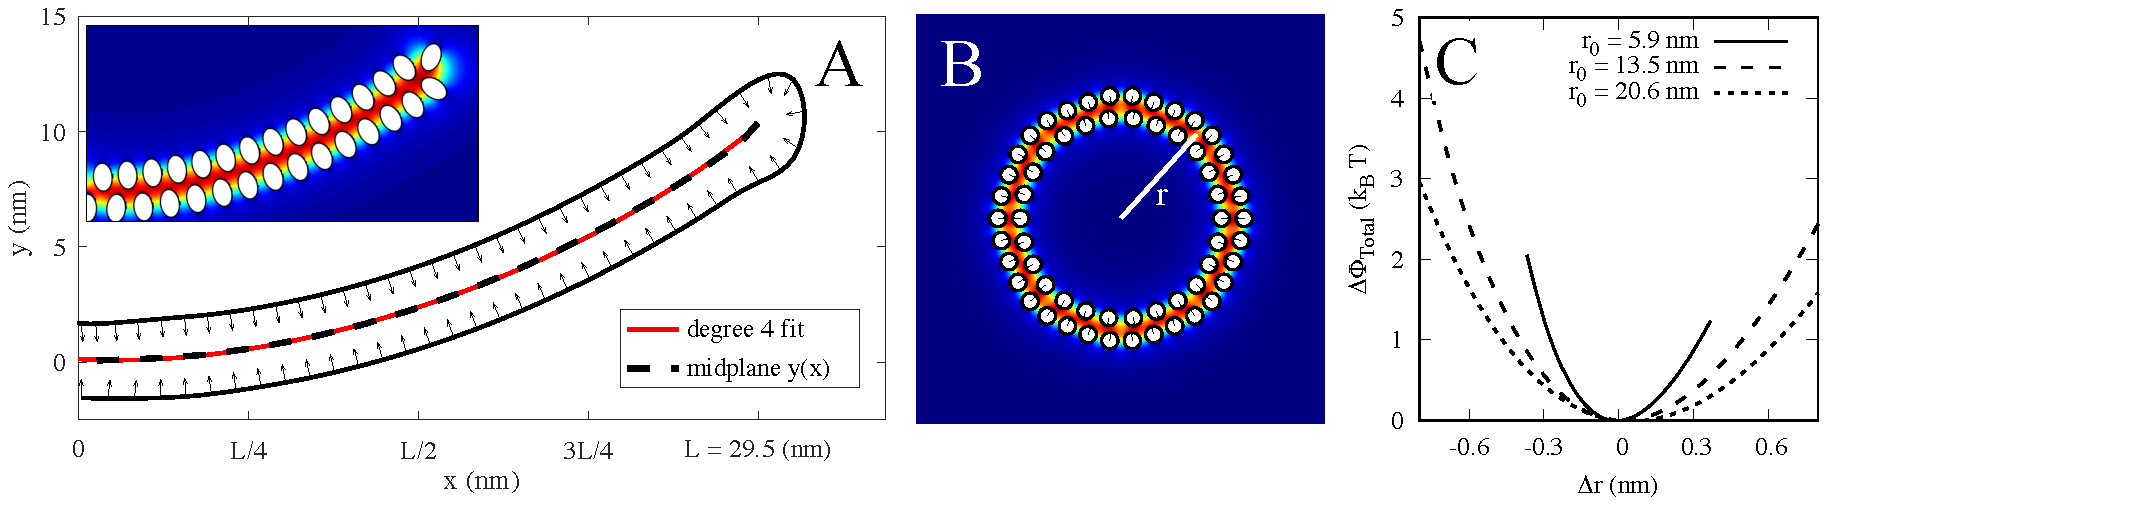
\includegraphics[width=\textwidth]{figures/SA1_fig2.pdf}
\end{center}\vspace{-1.em}
\caption{\footnotesize (A) A partially clamped bilayer with mid-plane (dashed curve) under uniform load.
The quartic fit comes from continuum theory. 
(B) A circular vesicle at equilibrium. (C) The area modulus derives
from convexity in energy as a function of radius. 
\label{fig:bend}}
\end{figure}

\subsubsection{Evidence for elastic properties}
\label{sssec:evidence}
We tested for elastic properties by subjecting two-dimensional bilayer morphologies
to external loads \cite{Fu19}, using realistic
values for phospholipid length \cite{Boal},
the screening length $\rho = 2.5$ nm \cite{Eriksson1989,Lin2005,Parsegian,Israelachvili80,TerziDeserno17}
and  interfacial tension $\gamma=4.1$ pN nm$^{-1}$  \cite{GarciaSaez, KUZMIN2005, Petelska2012}.
We first considered a planar bilayer subject to a uniform vertical load on the particle centers (Figure \ref{fig:bend}). 
The bilayer is clamped and horizontal at one end and the restoring force in the free part 
of the bilayer opposes the load. Twist and saddle splay are both zero, singling out splay
as the only distortion.
% In this situation, the directors are also parallel to the unit surface
%normal. As such $\Div \mathbf{d} = -2H$ where $H$ is the mean curvature of the surface. 
Since deformations are small \eqref{ansatz3}, it is possible to solve the bilayer loading in closed form. 
This analytical solution (red curve) basically overlaps the midplane of the particle based solution (Figure \ref{fig:bend}A). 

\begin{wrapfigure}[13]{l}{0.5\textwidth}
\centerline{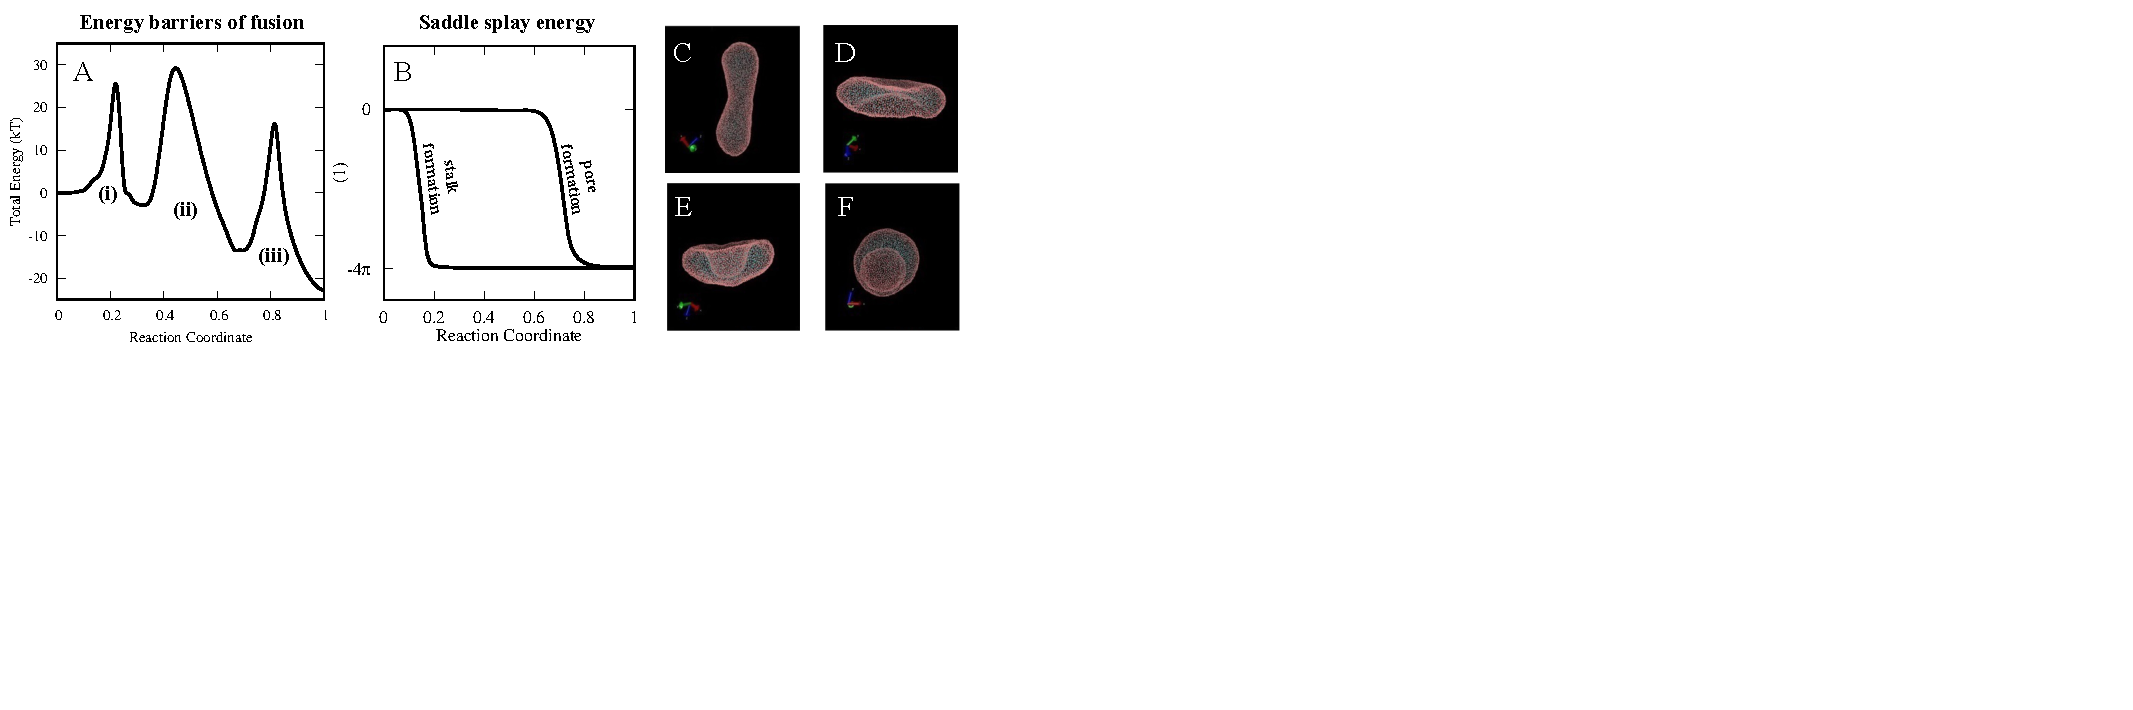
\includegraphics[width=0.5\textwidth]{figures/SA1_fig3.pdf}}
\caption{{\footnotesize (A) Energy barriers for stalk formation (i), hemifusion
diaphragm expansion (ii) and pore formation (iii). 
(B) Saddle-splay energy for each change in \emph{monolayer} topology
calculated in \cite{RyKlYaCo16}. (C)--(F): Shape transition of vesicle at different values of volume to area ratio from coarse-grained simulations of lipid bilayer membranes \cite{Fu16}.}}
\label{fig:barriers}
\end{wrapfigure}
Experimental measurements have accurately determined 
the bending modulus for several lipid types, with 
typical values lying around 10 \kBT\; \cite{Naetal15,VeBrPa15,NAGLE2000159,PhysRevLett.113.248102}.
By comparing with the exact solution, we derived a bending modulus
in the range 8.51 -- 13.54 \kBT, which is in 
excellent agreement with the experimentally derived value, especially considering how few parameters the HAP 
formalism involves. 

We also considered the stretching deformation \cite{Fu19}. 
Stretching occurs whenever there is an excess monolayer area,
and it is energetically costly since it exposes hydrocarbon tails to water. 
%Monolayers are not, strictly speaking, area incompressible,
%and 
Manipulation experiments give a monolayer area modulus in the range 
30 -- 40 \kBT\; nm$^{-2}$ \cite{Nagle17, Nagle17-2}. 
To measure an area modulus, we stretched a circular vesicle, modeling the cross-section 
of a bilayer tube (Figure \ref{fig:bend}B \& C).
%We then stretched the vesicle beyond and beneath equilibrium radius and recorded the change in energy. 
This procedure gave a monolayer area modulus 
34 $\pm$ 2 \kBT \;nm$^{-2}$, independently of the vesicle size, which
is also remarkably close to the experimental value.  

The successful outcomes of our preliminary tests suggest that the HAP particle configurations 
do behave like an elastic material. To validate our conjecture, we must consider 
ways to isolate or partially isolate the remaining distortions. 
The twist deformation, for example, has a modulus in the range of 1 to 2 \kBT\; 
as evaluated by molecular dynamics \cite{LeVeWa14}. 
But twist is mathematically zero in our two-dimensional monolayers,
and so we require a computationally efficient means for evaluating the 
boundary integral equations in a collection of three-dimensional particles. 
Specific Aim 2 discusses some of the outstanding implementation issues. 


Our eventual three-dimensional calculations must also consider the saddle-splay distortion,
and the calculations may help resolve some well-known issues in the theory \cite{TerziDeserno17}. 
Theoretical analysis of lipid phase transitions predict a negative saddle-splay modulus around $-8$ \kBT\;
\cite{SIEGEL2004366,SIEGEL20085200}.
This value, however, 
predicts an energy barrier for monolayer fusion on the order of 200  \kBT, which runs counter to 
the value 30 \kBT\; estimated in experiments \cite{RyKlYaCo16,FrRoPi17,Tran7106}.  
We expect the particle-based approach can shed light on this inconsistency. 



